%% ****** Start of file slactemplate.tex ****** %
%%
%%
%%   This file is part of the APS files in the REVTeX 4 distribution.
%%   Version 4.0 of REVTeX, August 2001
%%
%%
%%   Copyright (c) 2001 The American Physical Society.
%%
%%   See the REVTeX 4 README file for restrictions and more information.
%%
%
% This is a template for producing manuscripts for use with REVTEX 4.0
% Copy this file to another name and then work on that file.
% That way, you always have this original template file to use.
%
\documentclass[twocolumn,twoside,prd]{revtex4} %bktemp - prd -> slac
%\documentclass[preprint,twoside,prd]{revtex4} %bktemp - prd -> slac

\newif\ifpdf \ifx\pdfoutput\undefined \pdffalse \else \pdftrue \fi 
\ifpdf \usepackage[pdftex]{graphicx} \else \usepackage{graphicx} \fi 
\usepackage{fancyhdr}
\usepackage{amsmath}
\pagestyle{fancy}
\fancyhead{} % clear all fields
\fancyhead[C]{\it {}} \fancyhead[RO,LE]{\thepage}
\fancyfoot{} % clear all fields
\fancyfoot[LE,LO]{\bf {}}
\renewcommand{\headrulewidth}{0pt}
\renewcommand{\footrulewidth}{0pt}
\renewcommand{\sfdefault}{phv}
\newif\ifJASA \JASAfalse

%\setlength{\textheight}{235mm}
%\setlength{\textwidth}{170mm}
%\setlength{\topmargin}{-20mm}
%\renewcommand\topmargin{0in}
\def \pmiss {{\,/\!\!\!p}}
\def \met {{\,/\!\!\!\!E_{T}}}
\def \jj {\,2j}
\def \jjj {\,3j}
\def \jjjj {\,4j}
\def \jjjjj {\,5j}
\def \jjjjjj {\,6j}
\def \jjjjjjj {\,7j}
\def \figuresize {3.75in}
\newcommand {\footnoteIgnore}[1]{\footnote{#1}}
\newcommand {\footnoteParenthetical}[1]{\footnote{#1}}
\newcommand {\expBK}[1]{e^{#1}}
\newcommand {\abs}[1]{\left| #1 \right|}
\newcommand {\floor}[1]{\left\lfloor #1 \right\rfloor}
\renewcommand\topmargin{0in}

% You should use BibTeX and apsrev.bst for references

\thispagestyle{fancy}
%\bibliographystyle{unsrt}
\bibliographystyle{apsrev}

\def \Quaero {{\sc Quaero}}
\def \pythia {{\sc Pythia}}

\begin{document}

%Title of paper

\title{Optimal Binning for Likelihood Ratios}
\author{Bruce Knuteson}
\email{knuteson@mit.edu}
\homepage{http://mit.fnal.gov/~knuteson/}
\affiliation{Massachusetts Institute of Technology}

\author{Sheel Dandekar}
\email{sdandek@mit.edu}
\homepage{http://mit.fnal.gov/~knuteson/}
\affiliation{Massachusetts Institute of Technology}



\keywords{optimization, hypothesis testing, kernel density estimation}
\date{\today}

\begin{abstract}
A binned likelihood ratio provides a robust yet sensitive method for discriminating between two hypotheses.  But how should the bins be chosen?  Somewhat surprisingly, the literature does not yet appear to contain a satisfactory, general prescription for choosing an optimal binning.  This article suggests such a prescription, investigates its implications in several limiting cases, and provides examples of its use.   
\end{abstract}

%\maketitle must follow title, authors, abstract
\maketitle
\tableofcontents %bktemp

%===============================================================

\section{The problem}

Let us say that two scientists, Hanna and Barbera, each have a hypothesis about the occurrence of hurricanes along the coast of Florida.  Let us call Hanna's hypothesis $h$ and Barbera's hypothesis $b$.  Because of the complicated nature of hurricane modeling, both in terms of the large number of variables involved and the limitations on how well those variables can be measured, Hanna and Barbera each create a computer simulation based on their hypothesis.  Each run of the simulation outputs a hurricane with values for many variables, such as peak wind speed, where on the coast it strikes, rate at which the eye of the hurricane travels, duration of the hurricane, etc.  Both scientists run their simulations thousands of times to generate a large number of points, where each point contains information about dozens of parameters of a hurricane, and also has an associated weight.  Because the computer simulation creates many more hurricanes than actually occur, each point has a weight (not necessarily an integer), to denote how many hurricanes that point stands for.  
 
Dana, another researcher in Miami, has laboriously collected information about the peak wind speeds of hurricanes in Miami-Dade County, stretching back many years.  Let us call this data $d$, which is a set of wind speeds, $\{ d_l \}$. He wants to use $d$ to test which of Hanna and Barbara's hypotheses is more likely to be correct.  In order to do so, he creates a set of points for each simulation using the parameter of interest (peak wind speed).  Call the set of points from Hanna's and Barbera's simulations, which take the form (peak wind speed, associated weight), $\{ h_i \}$ and $\{ b_j \}$, respectively.  

The points $\{ h_i \}$ and $\{ b_j \}$ can be thought of as points chosen from their respective parent distributions,  $h(x)$ and $b(x)$.  Here x is some wind speed, and $h(x)dx$ and $b(x)dx$ are the number of hurricanes falling between  $x$ and $x+dx$ for small $dx$.  Unfortunately, Dana does not know the analytic form of the parent distribution, nor can the simulation even tell him the values of $h(x)$ and $b(x)$ for a particular wind speed.  All he has is a set of wind speeds, with weights, pulled from each parent distribution.

In order to approximate the parent distributions, Dana decides to choose a set of bins, which will divide the possible peak wind speeds into a number of regions.  For each of these bins, he wishes to construct a probability distribution $p(h_k)$, which equals the number of hurricanes expected in bin $k$ if $h$ is correct. (Throughout this article $i$ and $j$ are used to index the points drawn from $h$ and $b$, respectively, and $k$ is used to index bins.)  The width of the distribution $p(h_k)$ reflects uncertainty in the number of hurricanes predicted by $h$ with peak winds speeds within bin $k$, due to the limited statistics of $\{ h_i \}$; in the limit that bin $k$ contains many points, the number of hurricanes predicted by $h$ in bin $k$ is known very accurately, and $p(h_k)$ approaches a delta function.  Similarly, the points $\{ b_j \}$ can be turned into a prediction $p(b_k)$ for the number of hurricanes expected in bin $k$ if $b$ is correct.

The calculation of a binned likelihood can then be used to determine to what extent the data favors Hanna's or Barbera's hypothesis.  Often in the physical sciences the distribution of counts in each bin is Poisson; this is assumed in what follows.  In a particular bin $k$, the probability of observing $d_k$ hurricanes in the data assuming the correctness of $h$ is then

\begin{equation}
p(d_k|h) = \int_0^\infty{ \frac{ e^{-h_k} {h_k}^{d_k} }{ d_k! } p(h_k) \, dh_k }.
\end{equation}
Likewise, the probability of observing $d_k$ events in the data assuming the correctness of $b$ is given by
\begin{equation}
p(d_k|b) = \int_0^\infty{ \frac{ e^{-b_k} {b_k}^{d_k} }{ d_k! } p(b_k) \, db_k }.
\end{equation}
The probability of observing the entire data $d$, assuming the correctness of $h$ and neglecting correlated uncertainties among the predictions of $h$ in each bin, is
\begin{equation}
p(d|h) = \prod_k { p(d_k|h) }.
\end{equation}
Similarly,
\begin{equation}
p(d|b) = \prod_k { p(d_k|b) }.
\end{equation}
The binned likelihood ratio, a measure of the extent to which the data favors $h$ relative to $b$, is then
\begin{equation}
{\cal L} = \frac{ p(d|h) }{ p(d|b) }.
\end{equation}

{\em But how should the bins be chosen?}  Many finely spaced bins allow finer sampling of differences between the hypotheses $h$ and $b$, but introduce a larger uncertainty in the prediction within each bin.  A few coarsely spaced bins allow only coarse sampling of the distributions predicted by $h$ and $b$, but the predictions within each bin are more robust.  The question at hand is not only how many bins to use, but also where to place their edges.

\section{The solution}

Loosely speaking, bins should be used that maximally distinguish between the hypotheses $h$ and $b$.  We make this intuitive notion precise by proposing that the figure of merit ${\cal M}$ for choosing a given binning should be the expected evidence in favor of $h$ if $h$ is correct, plus the expected evidence in favor of $b$ if $b$ is correct.

The evidence $e$ in favor of $h$ (relative to $b$) provided by a particular set of data $d$ is taken to be~\cite{Jaynes}
\begin{equation}
e = \log{ \frac{ p(d|h) }{ p(d|b) } }.
\end{equation}
  The expected evidence in favor of $h$ if $h$ is correct, a quantity independent of data, is an average of the evidence over an ensemble of pseudo data samples distributed assuming the correctness of $h$.  Similarly, the expected evidence in favor of $b$ if $b$ is correct is an average of the evidence over an ensemble of pseudo data samples distributed assuming the correctness of $b$.

Given a particular choice of bins indexed by $k$, the proposed figure of merit is thus
\begin{multline}
\label{eqn:FigureOfMeritComplicated}
{\cal M} =  \sum_{d_1=0}^\infty \sum_{d_2=0}^\infty \cdots 
 \left( { p(d|h)  } \right) \times \\
 \log\left( \frac{p(d|h)}{p(d|b)}\right)  \\
 + \left( h \leftrightarrow b \right) - {\cal P}.
\end{multline}



In words, the initial $\sum_{d_1=0}^\infty \sum_{d_2=0}^\infty \cdots$ is a sum over all possible outcomes of the experiment; each bin $k$ in principle can contain any number of entries $d_k$.  These possible outcomes are weighted according to the probability of their occurrence $\prod_k{ p(d_k|h) }$ assuming the correctness of the hypothesis $h$.  If a particular outcome $\{ d_k \}$ is observed, than the evidence of those data in favor of $h$ will be $\log{\prod_k \frac{p(d_k|h)}{p(d_k|b)}}$.  The penultimate term $\left( h \leftrightarrow b \right)$ represents the analogous computation with $h$ and $b$ switched.  The final term ${\cal P}$ is a bias-removing penalty term.

The previous expression for ${\cal M}$ can be simplified: \footnoteIgnore{Straightforward interpretation of numerical results, as in Sec.~\ref{sec:Examples}, is facilitated by multiplying this expression for ${\cal M}$ by $(\log_{10}{e})/2$.}  

\begin{multline}
\label{eqn:FigureOfMeritComplicated}
{\cal M} =  \sum_{d_1=0}^\infty \sum_{d_2=0}^\infty \cdots 
  \prod_k{ p(d_k|h)  } \times \\
 \log \left( \prod_k \frac{p(d_k|h)}{p(d_k|b)} \right)  \\
 + ( h \leftrightarrow b) - {\cal P}.
\end{multline}


\begin{multline}
\label{eqn:FigureOfMeritComplicated2}
{\cal M}  = \sum_{d_1=0}^\infty \sum_{d_2=0}^\infty \cdots 
  \prod_{k=1}{ p(d_k|h)  } \times \\
 \sum_k \log \left( \frac{p(d_k|h)}{p(d_k|b)} \right)  \\
 + ( h \leftrightarrow b) - {\cal P}\\
\end{multline}

\begin{multline}
\label{eqn:FigureOfMeritComplicated3}
{\cal M}  =  \sum_{d_1=0}^\infty \sum_{d_2=0}^\infty \cdots 
   {p(d_1|h)} \times \prod_{k=2}{ p(d_k|h)  }   \times \\
 \left( \log \left( \frac{p(d_1|h)}{p(d_1|b)} \right) + \sum_{k=2} \log \left( \frac{p(d_k|h)}{p(d_k|b)} \right)\right)  \\
 +  ( h \leftrightarrow b  ) - {\cal P}\\      
\end{multline}

\begin{multline}
\label{eqn:FigureOfMeritComplicated4}
{\cal M}  =  \sum_{d_1=0}^\infty \sum_{d_2=0}^\infty \cdots 
   {p(d_1|h)} \times \prod_{k=2}{ p(d_k|h)  }   \times \sum_{k=2} \log \left( \frac{p(d_k|h)}{p(d_k|b)} \right)\\
 + \sum_{d_1=0}^\infty \sum_{d_2=0}^\infty \cdots   {p(d_1|h)} \times \prod_{k=2}{ p(d_k|h)  }  \times  \log \left( \frac{p(d_1|h)}{p(d_1|b)} \right)  \\
 +  ( h \leftrightarrow b  ) - {\cal P}\\        
\end{multline}

\begin{multline}
\label{eqn:FigureOfMeritComplicated5}
{\cal M}  =  \left(\sum_{d_1=0}^\infty {p(d_1|h)} \right) \times \sum_{d_2=0}^\infty \cdots \prod_{k=2}{ p(d_k|h)  }   \times \sum_{k=2} \log \left( \frac{p(d_k|h)}{p(d_k|b)} \right)\\
 + \sum_{d_1=0}^\infty  \left( {p(d_1|h)} \times  \log \left( \frac{p(d_1|h)}{p(d_1|b)} \right)\right)  \\ 
\times \left(\sum_{d_2=0}^\infty \cdots \prod_{k=2}{ p(d_k|h)  }\right)  
 +  ( h \leftrightarrow b  ) - {\cal P}\\        
\end{multline}

\begin{equation}
\label{eqn:FigureOfMeritComplicated6}
\sum_{d_k=0}^\infty {p(d_k|h)} = 1 \mbox{, so this simplifies to}
\end{equation}

\begin{multline}
\label{eqn:FigureOfMeritComplicated7}
{\cal M}  =  \sum_{d_2=0}^\infty \cdots \prod_{k=2}{ p(d_k|h)  } \times \sum_{k=2} \log \left( \frac{p(d_k|h)}{p(d_k|b)} \right)\\
 + \sum_{d_1=0}^\infty   {p(d_1|h)} \times  \log \left( \frac{p(d_1|h)}{p(d_1|b)} \right) \\ 
 +  ( h \leftrightarrow b  ) - {\cal P}\\       
\end{multline}

If we continue in this manner, we get 

\begin{multline}
\label{eqn:FigureOfMerit}
{\cal M} = \sum_k \sum_{d_k=0}^\infty \left( p(d_k|h) - p(d_k|b) \right)\times \\\left( \log{ p(d_k|h) } - \log{ p(d_k|b) } \right) - {\cal P}.
\end{multline}

This expression shows clearly that
\begin{itemize}
\item ${\cal M}$ is unchanged under the replacement $h \leftrightarrow b$;
\item neglecting the penalty term, ${\cal M} \geq 0$; and
\item neglecting the penalty term, ${\cal M} = 0$ if and only if $h$ and $b$ are identical.
\end{itemize}
The semi-positive-definiteness of ${\cal M}$ without the penalty term means that statistical fluctuations in the Monte Carlo points $\{ h_i \}$ and $\{ b_j \}$ make the expected value greater than zero, even if $h=b$.  The penalty term ${\cal P}$, a function of the number of bins and the number of events generated from $h$ and from $b$, but independent of the actual values of the points $\{ h_i \}$ and $\{ b_j \}$, is chosen so that the expected value of ${\cal M}$ is zero for equivalent hypotheses $h$ and $b$.  The computation of ${\cal P}$ in the limit of large statistics is discussed in Sec.~\ref{sec:PenaltyTerm}.

The main result of this article is the proposal that the binning for a likelihood ratio calculation should be chosen to maximize ${\cal M}$ in Eq.~(\ref{eqn:FigureOfMerit}).  Sec.~\ref{sec:SpecialCases} investigates this proposal in commonly encountered limits; Sec.~\ref{sec:Examples} provides examples of the practical use of this prescription; Sec.~\ref{sec:MultivariateCase} treats the multivariate case.


\section{\label{sec:SpecialCases}Special cases}

\subsection{Calculation of $p(h_k)$ and $p(b_k)$}

The calculation of the distributions $p(h_k)$ and $p(b_k)$ for the predicted number of events in bin $k$ from $h$ and $b$ requires knowledge of how the points $\{ h_i \}$ and $\{ b_j \}$ are drawn from the unknown distributions $h(x)$ and $b(x)$.  The points $\{ h_i \}$ may be drawn uniformly in $x$, for example, discarding a point if a second uniformly distributed random number exceeds the value of $h(x)$ at that point; this is a standard Monte Carlo technique.  Alternatively, the points $\{ h_i \}$ may be drawn uniformly in $x$, and each point assigned a weight proportional to the value of $h(x)$ at that point.  In general, then, the points $\{ h_i \}$ are weighted.

If the points $\{ h_i \}$ all have equal weight $w$, the calculation of $p(h_k)$ is straightforward.  Some integer $n_k$ of the points $\{ h_i \}$ fall into bin $k$, and $p(h_k)$ can be more properly written as $p(h_k|n_k,w)$. 

\begin{equation}
p(h_k|n_k,w) = p(n_k|h_k,w) \times \frac{p(h_k|w)}{p(n_k|w)}.
\end{equation}

where $p(h_k|w)$ and $p(n_k|w)$ are prior probabilities.  Assuming a flat prior for the number of events expected in bin $k$, $p(h_k|w)$ is constant.  $p(n_k|w)$ is also constant, and it is determined by the normalization condition

\[
\int_0^\infty p(h_k)\,d{h_k} = 1.
\]

$p(h_k|n_k,w)$ is then proportional to $p(n_k|h_k,w)$, which follows a Poisson distribution in $n_k$ with mean $h_k/w$.  Including the constant of proportionality,
\begin{equation}
p(h_k) = \frac{ e^{-(h_k/w)} (h_k/w)^{n_k} }{ w (n_k!) }.
\end{equation}
In the limit $n_k \gg 1$, this reduces to the familiar
\begin{equation}
\label{eqn:phkLargeStatistics}
p(h_k) \xrightarrow[n_k \gg 1]{} \frac{1}{\sqrt{2\pi}{\delta h_k}} \expBK{ - ( h_k - \hat h_k )^2 / 2 {\delta h_k}^2 },
\end{equation}
where $\hat h_k = w n_k$ is the mean of the Gaussian distribution, and $\delta h_k = w \sqrt{n_k}$ is the width.  The Gaussian distribution is valid up to a fractional error of order $1/{n_k}$. 

\subsection{Large statistics}

If Eq.~(\ref{eqn:phkLargeStatistics}) can be used to express $p(h_k)$ and $p(b_k)$, and if the expected number of events $\hat h_k$ and $\hat b_k$ in each bin $k$ is large compared to unity, the figure of merit ${\cal M}$ can be simplified.  Eqs. 1 and 2 go from Poisson to Gaussian in this limit, and summations over $d_k$ become integrals over $d_k$.   Substituting into Eq.~\ref{eqn:FigureOfMerit}:

%\ifJASA
%\begin{multline}
%\label{eqn:SimplifyM1}
%{\cal M} = \sum_k \int_0^\infty{ \left( \int_0^\infty{ \frac{1}{2\pi}{\delta h_k}{\sqrt{d_k}} \expBK{- \frac{( d_k -  h_k )^2}{ 2{d_k}} - \frac{( h_k - \hat h_k )^2} {2 {\delta h_k}^2} }  \, dh_k}  - ( h \leftrightarrow b  )\right) \times  (\log ( \int_0^\infty{ \frac{1}{2\pi}{\delta h_k}{\sqrt{d_k}}\expBK{- \frac{( d_k -  h_k )^2} {2 {d_k}} - \frac{( h_k - \hat h_k )^2} {2 {\delta h_k}^2} }  \, dh_k}) - \log( h \leftrightarrow b  )) \, dd_k} - {\cal P} \\
%\end{multline}
%\else
\begin{multline}
\label{eqn:SimplifyM1}
{\cal M} = \sum_k \int_0^\infty{ \left( \int_0^\infty{ \frac{1}{2\pi}{\delta h_k}{\sqrt{d_k}} \expBK{- \frac{( d_k -  h_k )^2}{ 2{d_k}} - \frac{( h_k - \hat h_k )^2} {2 {\delta h_k}^2} }  \, dh_k} \right. } \\
{\left. - (h \leftrightarrow b) \right) \times } \\
{ \left(\log \left( \int_0^\infty{ \frac{1}{2\pi}{\delta h_k}{\sqrt{d_k}}\expBK{- \frac{( d_k -  h_k )^2} {2 {d_k}} - \frac{( h_k - \hat h_k )^2} {2 {\delta h_k}^2} }  \, dh_k} \right) \right. } \\
{ \left.  - \log( h \leftrightarrow b  )\right) \, dd_k} - {\cal P} \\
\end{multline}
%\fi

\ifJASA
\begin{multline}
\label{eqn:SimplifyM2}
{\cal M} = \sum_k \int_0^\infty{  (\frac{1}{\sqrt{2\pi}}  \frac{1}{{d_k} + {\delta h_k}^2}  \expBK{- \frac {( d_k -  \hat h_k )^2} {2*({d_k} + {\delta h_k}^2)}} - ( h \leftrightarrow b)) \times (-\frac{1}{2}) (\log({d_k} + {\delta h_k}^2)  + \frac {( d_k -  \hat h_k )^2}{2*({d_k} + {\delta h_k}^2)} - \log( h \leftrightarrow b  )) \, dd_k} - {\cal P} \\
\end{multline}
\else
\begin{multline}
\label{eqn:SimplifyM2}
{\cal M} = \sum_k \int_0^\infty{  \left(\frac{1}{\sqrt{2\pi}}  \frac{1}{{d_k} + {\delta h_k}^2}  \expBK{- \frac {( d_k -  \hat h_k )^2} {2*({d_k} + {\delta h_k}^2)} }  \right. }  \\   
{ \left.   - ( h \leftrightarrow b)\right) \times \left(-\frac{1}{2}\right) } \\
{ \left(\log({d_k} + {\delta h_k}^2)  + \frac {( d_k -  \hat h_k )^2}{2({d_k} + {\delta h_k}^2)} - \log( h \leftrightarrow b  )\right) \, dd_k} - {\cal P} \\
\end{multline}
\fi


In this form, this integral is a difficult one to evaluate, owing to the presence of a $d_k$ term in the sigma term of the Gaussians.  We would like this to be constant, so that we can more easily integrate.  Therefore the approximation $d_k$ = $\hat h_k,\hat b_k$  is suggested to eliminate these $d_k$ terms.  The Gaussians are peaked at $\hat h_k$ and $\hat b_k$, respectively, so this is a possible approximation, but what is the magnitude of the error introduced by this approximation?

Considering the calculation of M for only a single bin, we found the error of the approximation for a couple sample distributions.  For $\hat h_k$ = 1000, $\hat b_k$ = 1100, $\delta h_k$ = 10, $\delta b_k$ = 10, the error was about 4 parts in 1000.  For $\hat h_k$ = 1000, $\hat b_k$ = 1100, $\delta h_k$ = 1, $\delta b_k$ = 1, the error was about 5 parts in 1000.  From these calculations we estimate the error to be smaller than leading by order ${\cal O}(\frac{1}{\hat h_k}, \frac{1}{\hat b_k})$. 

Another way to verify the approximation is to calculate the error using a Taylor series expansion.  In this expansion, we drop the log terms and only consider one the exponentials, since we are only concerned about the order of the error.  Let us call this new quantity $\cal N$.

\begin{multline}
\label{eqn:Taylor1}
{\cal N} = \int_0^\infty {\left( \frac{1}{\sqrt{2\pi}} \frac {1}{\sqrt{d_k +(\delta h_k)^2}} e^{- \frac {(d_k - \hat h_k)^2} {2(d_k +(\delta h_k)^2)}}\right)} \\ {\left(- \frac {1}{2} \right) \left( \frac {(d_k - \hat h_k)^2} {(d_k +(\delta h_k)^2)} + \frac {(d_k - \hat b_k)^2} {(d_k +(\delta b_k)^2)} \right) \, dd_k}  \\
\end{multline}

We can rewrite $d_k$ in the following manner:

\begin{equation}
\label{eqn:Taylor2}
d_k = h_k\left(1 - \frac {\hat h_k - d_k} {\hat h_k}  \right)
\end{equation}

The fractional term is considered to be small, and from here we will denote it as $\epsilon_h$.  Similarly, $d_k$ can be written in terms of $\hat b_k$ and a small term denoted as $\epsilon_b$.  The first term, which contains $\hat h_k$'s and multiplies the exponential, integrates to the same thing as in the case of the approximation.  This leaves us only one other term, which can be decomposed into a quadratic plus a constant term times the exponential.

\begin{multline} 
\label{eqn:Taylor3}
quadratic = \frac {1}{2} \left( \frac {\hat h_k + (\delta h_k)^2} {\hat b_k + (\delta b_k)^2} \right) \left(\frac {1-\epsilon_h}{1-\epsilon_b}  \right)
\end{multline}

\begin{multline} 
\label{eqn:Taylor4}
cosntant = \frac {1}{2} \left( \frac {(\hat h_k - \hat b_k)^2} {\hat b_k + (\delta b_k)^2} \right) \frac {1}{1-\epsilon_b}
\end{multline}

Assuming that $\epsilon_h$ is about equal to $\epsilon_b$, then the quadratic term is the same as in the approximation.  The constant term has an extra factor of $ \frac {1}{1-\epsilon_b}$.  This can be simplified:

\begin{equation} 
\label{eqn:Taylor5}
\frac {1}{1-\epsilon_b} = 1+\epsilon_b = 1 + \frac {\hat b_k - d_k}{\hat b_k}.
\end{equation}

Therefore the error term here is smaller than leading by a factor of $\frac {1}{\hat b_k}$, and the overall error term is order ${\cal O}(\frac{1}{\hat h_k}, \frac{1}{\hat b_k})$. 

After the approximation:   

\begin{multline}
\label{eqn:SimplifyM3}
{\cal M} = \sum_k \int_0^\infty{  \left(\frac{1}{\sqrt{2\pi}}  \frac{1}{{\hat h_k} + {\delta h_k}^2} \expBK{- \frac{( d_k -  \hat h_k )^2} {2*({\hat h_k} + {\delta h_k}^2)}}  - ( h \leftrightarrow b)\right) \times } \\
{ \left(-\frac{1}{2}\right) \left(\log({h_k} + {\delta h_k}^2)  + \frac {( d_k -  \hat h_k )^2}{2({h_k} + {\delta h_k}^2)} - \log ( h \leftrightarrow b  )\right) \, dd_k} - {\cal P}\\
\end{multline}

We can get rid of the log terms, because their contributions after being multiplied by each of the Gaussians and integrated will cancel to 0.  After integrating,

\begin{multline}
\label{eqn:SimplifyM4}
{\cal M} = \sum_k \frac {-1}{2} \left(\frac {\hat h_k + {\delta h_k}^2} {\hat h_k + {\delta h_k}^2} - \frac {(\hat h_k - \hat b_k)^2 + \hat b_k + {\delta b_k}^2 }{\hat h_k + {\delta h_k}^2} \right. \\
\left. - \frac {(\hat h_k - \hat b_k)^2 + \hat h_k + {\delta h_k}^2 }{\hat b_k + {\delta b_k}^2} + \frac {\hat b_k + {\delta b_k}^2}{\hat b_k + {\delta b_k}^2}\right) - {\cal P}\\
\end{multline}

\begin{multline}
\label{eqn:SimplifyM5}
{\cal M} = \sum_k \frac {-1}{2 (\hat h_k+ {\delta h_k}^2)(\hat b_k + {\delta b_k}^2)} \times \\ 
\left(-2 (\hat h_k+ {\delta h_k}^2)(\hat b_k + {\delta b_k}^2) \right. \\
\left. + (\hat h_k - \hat b_k)^2 ({h_k} + {\delta h_k}^2 + {b_k} + {\delta b_k}^2) \right. \\
\left. + ({h_k} + {\delta h_k}^2) + ({b_k} + {\delta b_k}^2)\right) - {\cal P}\\
\end{multline}

\ifJASA
\begin{multline}
\label{eqn:FigureOfMeritLargeStatistics}
{\cal M} \rightarrow
\sum_k \frac{1}{ 2(\hat h_k+{\delta h_k}^2)(\hat b_k + {\delta b_k}^2) } 
  \left( (\hat h_k-\hat b_k)^2 (\hat h_k + {\delta h_k}^2 + \hat b_k + {\delta b_k}^2) \right)
 \\ \left. + ((\hat b_k+{\delta b_k}^2) - (\hat h_k+{\delta h_k}^2))^2 \right) 
+ O\left(\frac{1}{\hat h_k}\, , \, \frac{1}{\hat b_k}\right) - {\cal P},
\end{multline}
\else
\begin{multline}
\label{eqn:FigureOfMeritLargeStatistics}
{\cal M} \rightarrow
\sum_k \frac{1}{ 2(\hat h_k+{\delta h_k}^2)(\hat b_k + {\delta b_k}^2) } \times \\
  \left( (\hat h_k-\hat b_k)^2 (\hat h_k + {\delta h_k}^2 + \hat b_k + {\delta b_k}^2) \right. \\
 \left. + ((\hat b_k+{\delta b_k}^2) - \left(\hat h_k+{\delta h_k}^2)\right)^2 \right) \\
+ O\left(\frac{1}{\hat h_k}\, , \, \frac{1}{\hat b_k}\right) - {\cal P},
\end{multline}
\fi
neglecting terms smaller than leading by order $1/{\hat h_k}$ and $1/{\hat b_k}$.

\subsection{\label{sec:PenaltyTerm}Penalty term}

The penalty term ${\cal P}$ is determined by requiring the expected value of the figure of merit $\langle {\cal M} \rangle$ under fluctuations in the Monte Carlo events to vanish, taking the true predictions $h$ and $b$ to be the same (so that $\langle \hat h_k \rangle = \langle \hat b_k \rangle$).  ${\cal P}$ thus depends only on the weights of the points $\{ h_i \}$ and $\{ b_j \}$, the number of points, and the number of bins, and is independent of the actual points $\{ h_i \}$ and $\{ b_j \}$.  The penalty term therefore in no way affects the placement of bins.  However, through its dependence on the number of bins, the penalty term does determine when placing additional bins is no longer to our advantage.

The dependence of ${\cal P}$ on the weights, the number of points, and the number of bins factorizes into three pieces:
\begin{equation}
\label{eqn:PenaltyTerm}
{\cal P} = {\cal P}_w {\cal P}_{n_\text{MC}} {\cal P}_{n_\text{bins}}.
\end{equation}
${\cal P}_w$, which sets the overall scale of ${\cal P}$, is determined by computing the expected value $\langle {\cal M} \rangle$ under fluctuations in the Monte Carlo points for a single bin encompassing the entire sample.  In the limit of large Monte Carlo statistics and large numbers of expected events, such that Eq.~(\ref{eqn:FigureOfMeritLargeStatistics}) holds, and if events from hypotheses $h$ and $b$ have been generated with uniform weights $w_h$ and $w_b$, then from Eq.~(\ref{eqn:FigureOfMeritLargeStatistics}) and ignoring terms smaller than leading by order $1/\hat h_k$ and $1/\hat b_k$,
\begin{multline}
\label{eqn:PenaltyTermWComplicated1}
{\cal P}_w = \frac {1} { 2(\hat h_k+{\delta h_k}^2)(\hat b_k + {\delta b_k}^2) }\\  
\times \left(\langle (\hat h_k-\hat b_k)^2 \rangle(\hat h_k + {\delta h_k}^2 + \hat b_k + {\delta b_k}^2) \right. \\
 \left. + \langle ((\hat b_k+{\delta b_k}^2) - (\hat h_k+{\delta h_k}^2))^2 \rangle \right)
\end{multline}

The only terms we need to find the expected value of is those terms that evaluate to 0, but due to fluctuations in the Monte Carlo events, will be non-zero.  These fluctuations in the Monte Carlo events are not large enough to change the expectation value of the terms that do not evaluate to 0.
\begin{equation}
\label{eqn:PenaltyTermWComplicated2}
\langle (\hat h_k-\hat b_k)^2 \rangle = \langle (\hat h_k-\hat b_k) \rangle^2 +  \delta (\hat h_k-\hat b_k)^2
\end{equation}
\begin{equation}
\label{eqn:PenaltyTermWComplicated2}
\langle (\hat h_k-\hat b_k)^2 \rangle = (\delta \hat h_k)^2 + (\delta \hat b_k)^2
\end{equation}

Similarly,

\begin{equation}
\label{eqn:PenaltyTermWComplicated3}
\langle ((\hat b_k+{\delta b_k}^2) - (\hat h_k+{\delta h_k}^2))^2 \rangle = n_k^h(w_h+w_h^2)^2 +  n_k^b(w_b+w_b^2)^2 
\end{equation}

Dropping terms smaller than leading by order $1/\hat h_k$ and $1/\hat b_k$,
\begin{multline}
\label{eqn:PenaltyTermWComplicated4}
{\cal P}_w = \frac {1}{2(\hat h_k+{\delta h_k}^2)(\hat b_k+{\delta b_k}^2)} \\
\times [((\delta h_k)^2 + (\delta b_k)^2)( \hat h_k +(\delta h_k)^2 + \hat b_k +(\delta b_k)^2)]
\end{multline}

Setting $\hat h_k$ = $\hat b_k$,
\begin{equation}
\label{eqn:PenaltyTermWComplicated5}
{\cal P}_w = \frac {1}{2 \hat {h_k}^2(1+w_h)(1+w_b)} [\hat {h_k}^2(w_h+w_b)(2+w_h+w_b)]
\end{equation}
 
\begin{equation}
\label{eqn:PenaltyTermWComplicated}
{\cal P}_w = \frac{(w_h+w_b)(2+w_h+w_b)}{2(1+w_h)(1+w_b)}.
\end{equation}
If the weights of events from $h$ and $b$ are equal ($w=w_h=w_b$), this is simply
\begin{equation}
\label{eqn:PenaltyTermWSimple}
{\cal P}_w = \frac{2 w}{1+w},
\end{equation}
a trivial function of the weight.

The factor ${\cal P}_{n_\text{MC}}$ results from our optimization over the large number of places at which bins can be split, and the factor ${\cal P}_{n_\text{bins}}$ results from the way in which this large number of places changes as additional bins are added.  ${\cal P}_{n_\text{MC}}$ and ${\cal P}_{n_\text{bins}}$ are determined empirically from an ensemble of samples as a function of the number of Monte Carlo points $n_\text{MC}$ and the number of bins $n_\text{bins}$.  When the iterative algorithm described in Sec.~\ref{sec:Examples} is used to place the bin edges, the results can be parametrized in the form
\begin{gather}
{\cal P}_{n_\text{MC}} = \frac{1}{2} \log_e ( 10 \, {n_\text{MC}} \, w ) \\
{\cal P}_{n_\text{bins}} = n_\text{bins}.
\end{gather}
The scaling of ${\cal P}_{n_\text{MC}}$ with ${n_\text{MC}}w$ is strikingly consistent, holding over five orders of magnitude from $10 \lesssim {n_\text{MC}} w \lesssim 10^6$.  ${\cal P}_{n_\text{bins}}$ is found to be simply proportional to the number of bins.

The above formulae for ${\cal P} = {\cal P}_w {\cal P}_{n_\text{MC}} {\cal P}_{n_\text{bins}}$ are strictly only appropriate when the points $\{ h_i \}$ and $\{ b_j \}$ have uniform weights, in the high statistics limit of Eq.~(\ref{eqn:FigureOfMeritLargeStatistics}), and when the iterative algorithm described in Sec.~\ref{sec:Examples} is used to determine the placement of bin edges.  In practice, since the only effect of the penalty term is to limit the number of bins placed, these expressions are generally applicable.  When in doubt, the penalty term can be calculated by drawing points for pseudo hypotheses $h$ and $b$ uniformly from the unit interval, with weight distributions equal to those of $\{ h_i \}$ and $\{ b_j \}$, applying the desired optimization procedure for determining bin placement, and evaluating $\langle {\cal M} \rangle$, averaged over this ensemble.

\subsection{Signal + background}

Consider a hypothesis $h$ composed of signal $s$ added to the background $b$, so that $h=b+s$.  The sample is divided into two bins, bin 1 and bin 2.  If the signal is small and localized to bin $2$, then $\hat h_1=\hat b_1+\hat s_1\approx \hat b_1$ and $\hat h_2 = \hat b_2 + \hat s_2$.  That is, the number of events $\hat h_1$ in bin 1 predicted by $h$ is equal to the expected background $\hat b_1$ plus the (negligible) expected signal $\hat s_1$, and the number of events $\hat h_2$ in bin 2 predicted by $h$ is equal to the expected background $\hat b_2$ plus the (non-negligible) expected signal $\hat s_2$.  In the large statistics limit of Eq.~(\ref{eqn:FigureOfMeritLargeStatistics}), ignoring the error $\delta s_2$ and terms smaller than leading by $1/b_2$, the figure of merit reduces to
\begin{equation}
{\cal M} \rightarrow \frac{ {\hat s_2}^2 (2 (\hat b_2 + {\delta b_2}^2) + \hat s_2) }{ 2 (\hat b_2 + {\delta b_2}^2)(\hat b_2 + {\delta b_2}^2 + \hat s_2) } - {\cal P}.
\end{equation}
Dropping the subscripts and hats on $\hat s_2$, $\hat b_2$, and $\delta b_2$ in order to connect with a familiar result, we note that if $s \ll b$, 
\begin{equation}
{\cal M} \rightarrow s^2/(b+{\delta b}^2) - {\cal P};
\end{equation}
and if $s \gg b$, 
\begin{equation}
{\cal M} \rightarrow s^2/2(b+{\delta b}^2) - {\cal P}.
\end{equation}
In either limit, since the penalty term ${\cal P}$ is independent of $s$, $b$, and $\delta b$, the maximization of the figure of merit ${\cal M}$ reduces to the maximization of the familiar $s/\sqrt{b+{\delta b}^2}$.  In the limit ${\delta b}^2 \ll b$, this reduces to the perhaps even more common $s/\sqrt{b}$.

\section{\label{sec:Examples}Examples}

Although in principle maximizing ${\cal M}$ requires optimizing the positions of all bin edges simultaneously, in practice it is convenient to choose the bin edges sequentially.  Starting with a single bin encompassing all points, this bin is split into two bins at a location chosen to maximize ${\cal M}$.  One of the two resulting bins is then split at a location chosen to maximize ${\cal M}$, and so on, until further division results in negligible or negative change in ${\cal M}$.

\subsection{Example \#1:  A bump}

An example of this procedure is shown in Fig.~\ref{fig:Example1}.  Figure~\ref{fig:Example1}(a) shows the true (unknown) distributions 
\begin{equation}
\begin{split}
h(x) = & \frac{n_b}{\lambda} e^{(-x/\lambda)} + \frac{n_s}{\sqrt{2\pi}\sigma}e^{(-(x-\mu)^2/2\sigma^2)}  \nonumber \\
b(x) = & \frac{n_b}{\lambda} e^{(-x/\lambda)}, \nonumber
\end{split}
\end{equation}
with parameters $n_b = 100$, $n_s=10$, $\lambda=10$, $\mu=20$, and $\sigma=5$.  The units on the vertical axis are the number of events expected in the data per unit $x$.  One thousand points have been randomly drawn from $b(x)$, each with weight 0.1, so that $1000\times0.1=100 = n_b = \int_0^\infty{b(x)\,dx}$.  Eleven hundred points have been randomly drawn from $h(x)$, each again with weight 0.1, so that $1100\times0.1 = 110 = n_b+n_s = \int_0^\infty{h(x)\,dx}$.  These points are displayed in Fig.~\ref{fig:Example1}(b), in bins of unit width in $x$.  Treating the range $0<x<\infty$ as a single bin, the initial figure of merit is calculated to be ${\cal M} = 0.05$.

\begin{figure}[htb]
\resizebox{\figuresize}{!}{\hskip -0.5cm \ifpdf 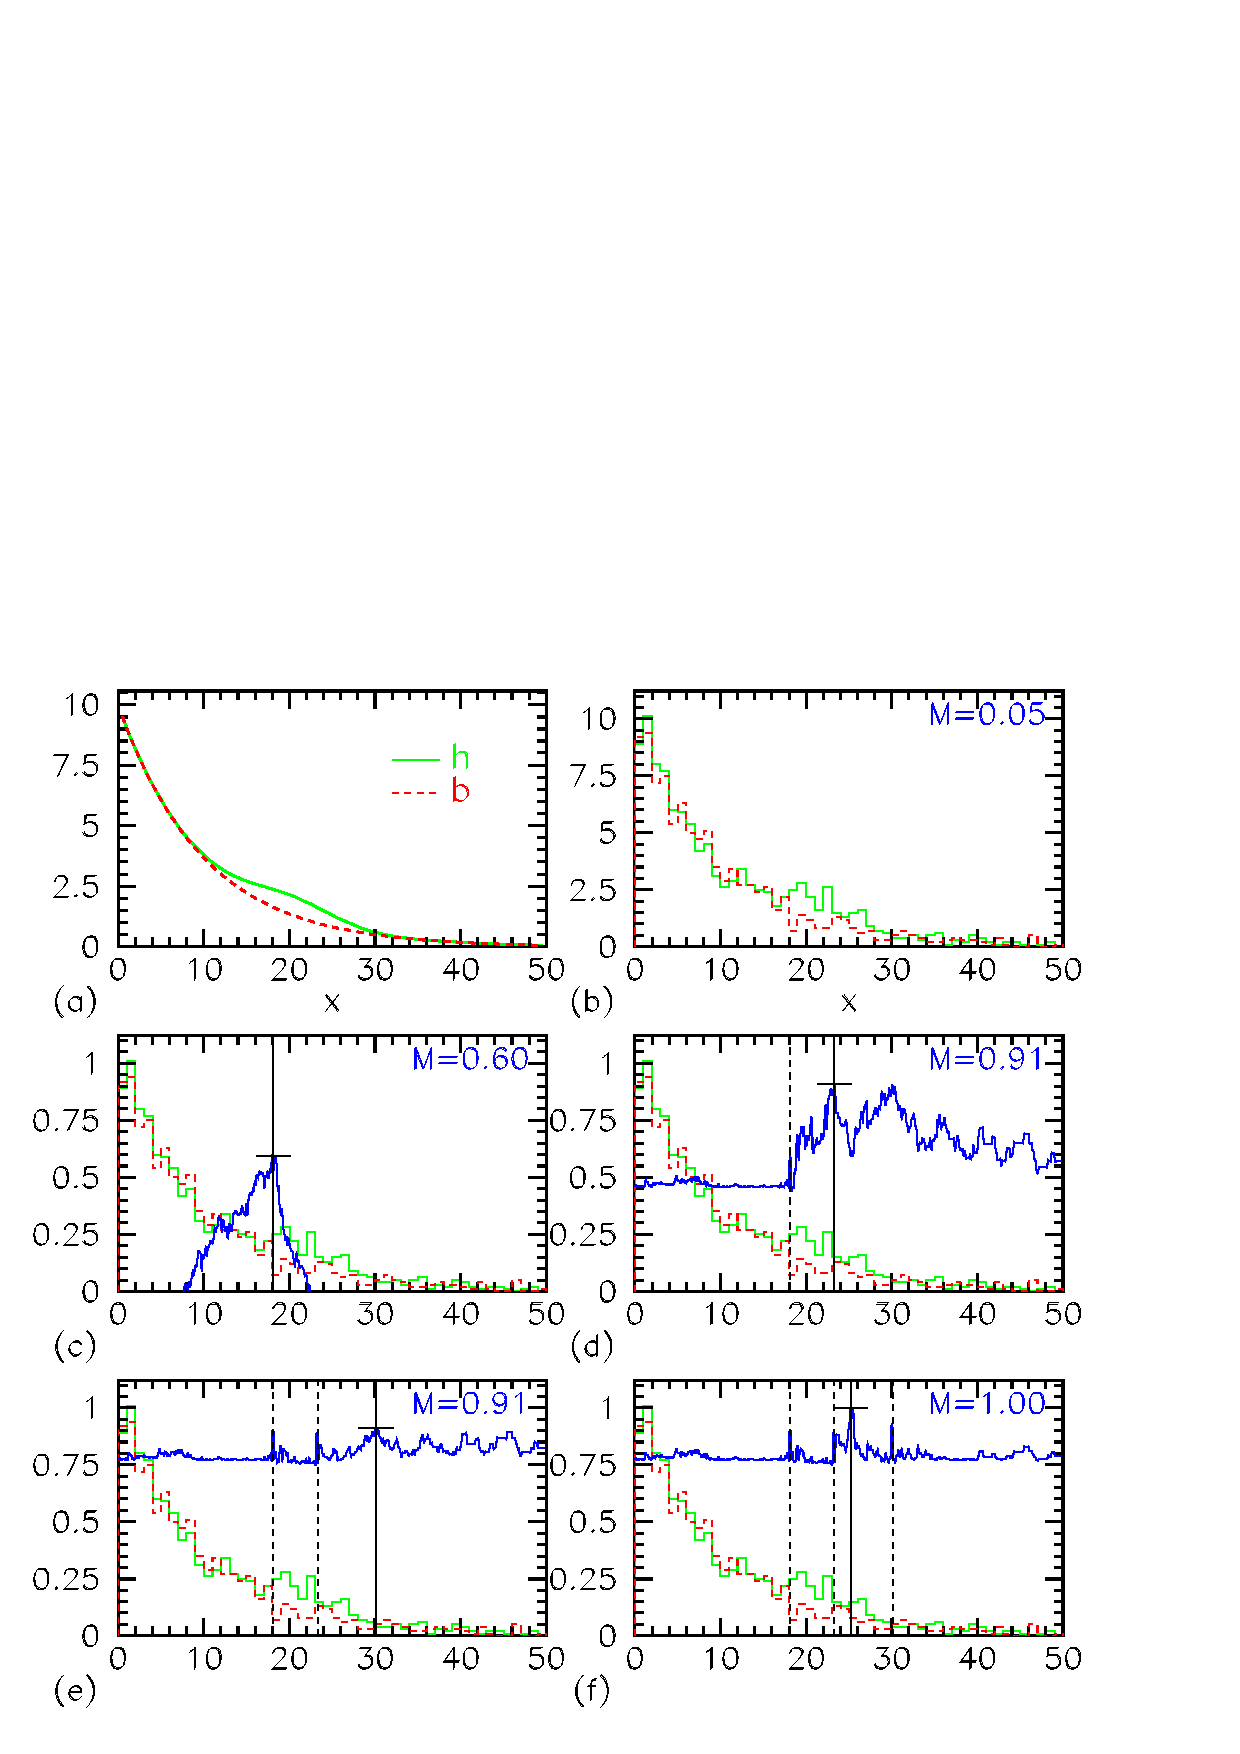
\includegraphics{figures/plot01.pdf} \else 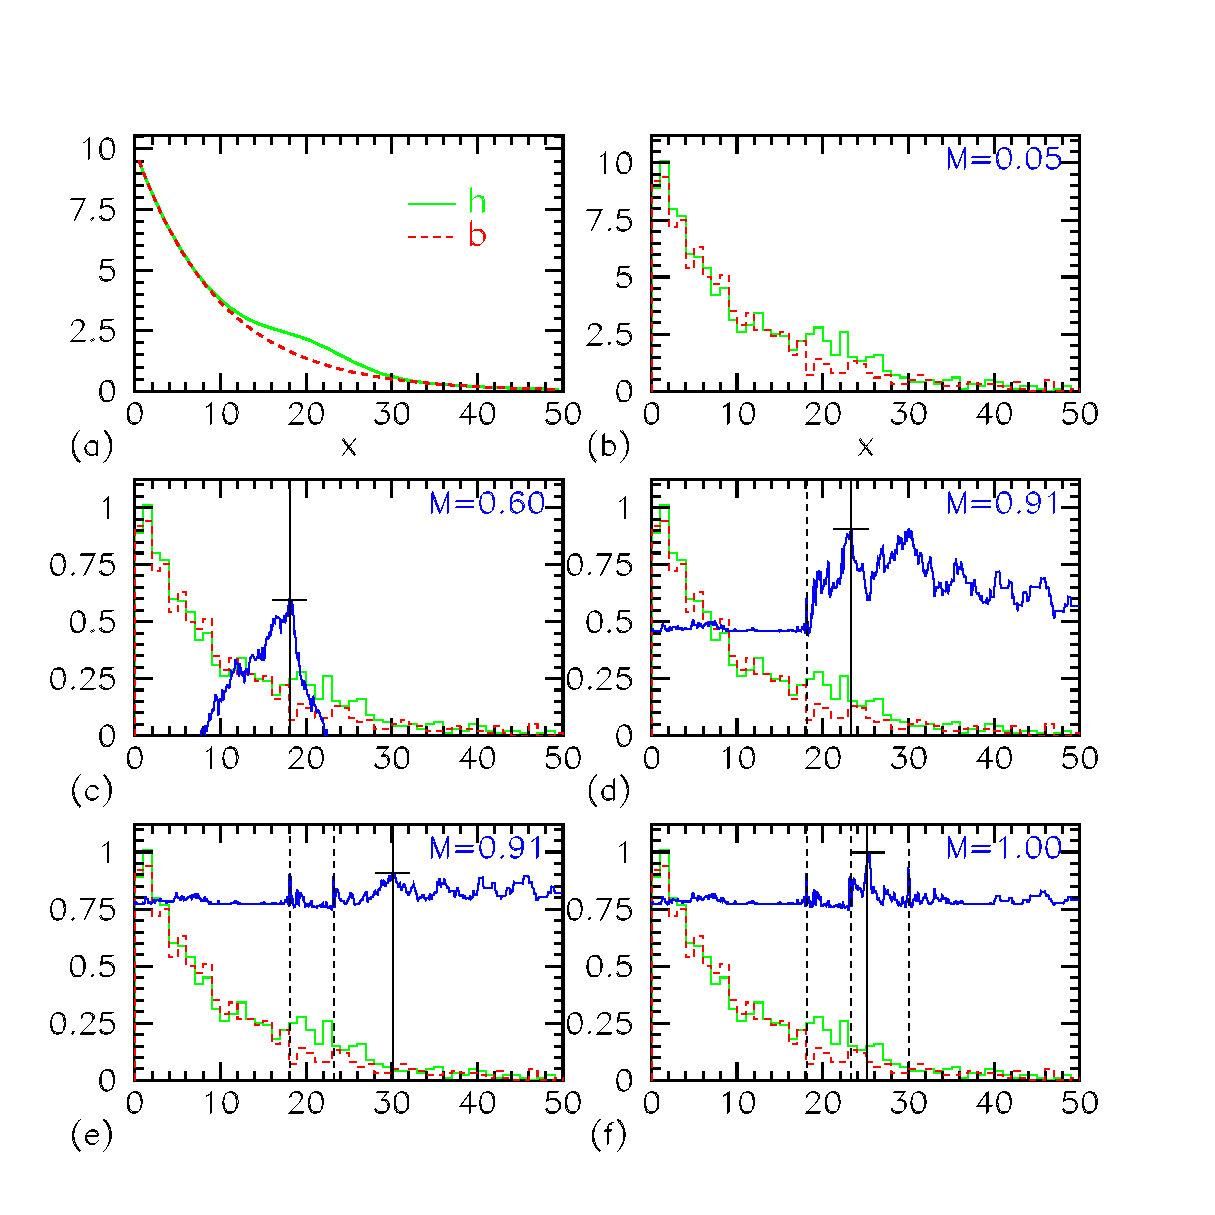
\includegraphics{figures/plot01.eps} \fi }
\vskip -0.2in 
\caption{An example of using ${\cal M}$ to choose a reasonable set of bins.  The analytical predictions (a) of $h$ (solid) and $b$ (dashed) are unknown, but are estimated (b) with Monte Carlo.  The vertical axis in (a) and (b) represents the number of data points expected per unit of $x$; the vertical axis in (c)--(f) has units of evidence, and represents the figure of merit ${\cal M}$ if an additional bin edge is placed at $x$.  Figures (c)--(f) show the successive placing of bin edges at maximal points of ${\cal M}$.}
\label{fig:Example1}
\end{figure}

The units on the vertical axis in Figs.~\ref{fig:Example1}(c)--(f) are expected evidence; the histograms of Fig.~\ref{fig:Example1}(b) have been superimposed with arbitrary scale.  The jagged curve marks the figure of merit ${\cal M}$ if a bin edge is added at location $x$.  Figure~\ref{fig:Example1}(c) shows the choosing of the first partition, with the figure of merit reaching an obvious maximum of 0.60 at $x=18.1$.  The choice of the second partition is shown in Fig.~\ref{fig:Example1}(d), with placement at $x=23.1$ narrowly winning out over a second local maximum at $x\approx 30$, improving the figure of merit to 0.91.  This second local maximum at $x=30.1$ is the choice for the third partition, shown in Fig.~\ref{fig:Example1}(e), the improvement barely exceeding the penalty term for adding an additional bin.  This third partition presents an opportunity not present before to isolate a region with $h\approx b$ around $x\approx 25$ from regions on either side with $h > b$, and some gain is achieved by placing a fourth partition at $x=25.2$.  Placing additional bins causes ${\cal M}$ to decrease, so the algorithm halts at a final figure of merit ${\cal M} = 1.00$.

The reasonable placement of bin choices in this example is somewhat striking.  The first two partitions immediately carve out the interval $18 < x < 23$ in which $h$ and $b$ differ most significantly.  The final two partitions refine the binning within the region $23<x<30$.   The bulk of the distribution at $x<18$ is completely ignored, as is the low statistics tail at $x>30$.  The penalty term of Eq.~(\ref{eqn:PenaltyTerm}) halts the subdivision of bins at a reasonable number.  Although the detailed bin placement naturally changes when different Monte Carlo points $\{ h_i \}$ and $\{ b_j \}$ are drawn from $h(x)$ and $b(x)$, the general pattern remains remarkably consistent.

The final figure of merit ${\cal M} = 1.0$ has an immediate and intuitive interpretation.  (For convenience of analytic expression, the figure of merit in the preceding sections is the sum of expected evidences for $h$ and $b$, with evidence expressed in terms of the natural logarithm.  For convenience of numerical interpretation, the figure of merit here is the average of the expected evidences, expressed in terms of the decimal logarithm.  The difference is simply an overall factor of $(\log_{10}{e})/2$.)  Speaking loosely, the expected result from actually performing the experiment should be that the data favors one hypothesis over the other by a factor of $\approx 10^{1.0} \approx 10$.  Speaking somewhat more precisely, if the experiment is performed many times and the average of the log of the likelihood ratio calculated in each experiment is taken, this average will be $\approx \pm 1.0$, the sign depending upon whether $h$ or $b$ is in fact correct.

%Running an ensemble of $10^4$ pseudo experiments confirms this result.  When the pseudo data are pulled from $b$, the mean evidence supporting $b$ is 0.63; when the pseudo data are pulled from $h$, the mean evidence supporting $h$ is 1.10.  The average of the means is 0.86, in reasonable agreement with the calculated figure of merit.  The difference results from the fact that the ensemble of pseudo experiments is distributed according to the true $h$ and $b$, while the figure of merit must be calculated from the given points $\{ h_i \}$ and $\{ b_j \}$.  

\subsection{Example \#2:  Gaussians of different widths}

A second illustrative example concerns the case in which $h$ and $b$ predict Gaussian distributions of different widths.  Figure~\ref{fig:Example2}(a) shows the true (unknown) distributions 
\begin{equation}
\begin{split}
h(x) = & \frac{n}{\sqrt{2\pi}{\sigma_h}}e^{(-(x-\mu)^2/2{\sigma_h}^2)} \nonumber \\
b(x) = & \frac{n}{\sqrt{2\pi}{\sigma_b}}e^{(-(x-\mu)^2/2{\sigma_b}^2)}, \nonumber 
\end{split}
\end{equation}
with parameters $n = 100$, $\mu=25$, $\sigma_h=5$, and $\sigma_b=8$.  The units on the vertical axis are again the number of events expected in the data per unit $x$.  One thousand points have been randomly drawn from $b(x)$ and from $h(x)$, each with weight 0.1.  These points are shown in the histogram in Fig.~\ref{fig:Example2}(b), in bins of unit width in $x$.  

\begin{figure}[htb]
\resizebox{\figuresize}{!}{\hskip -0.5cm \ifpdf 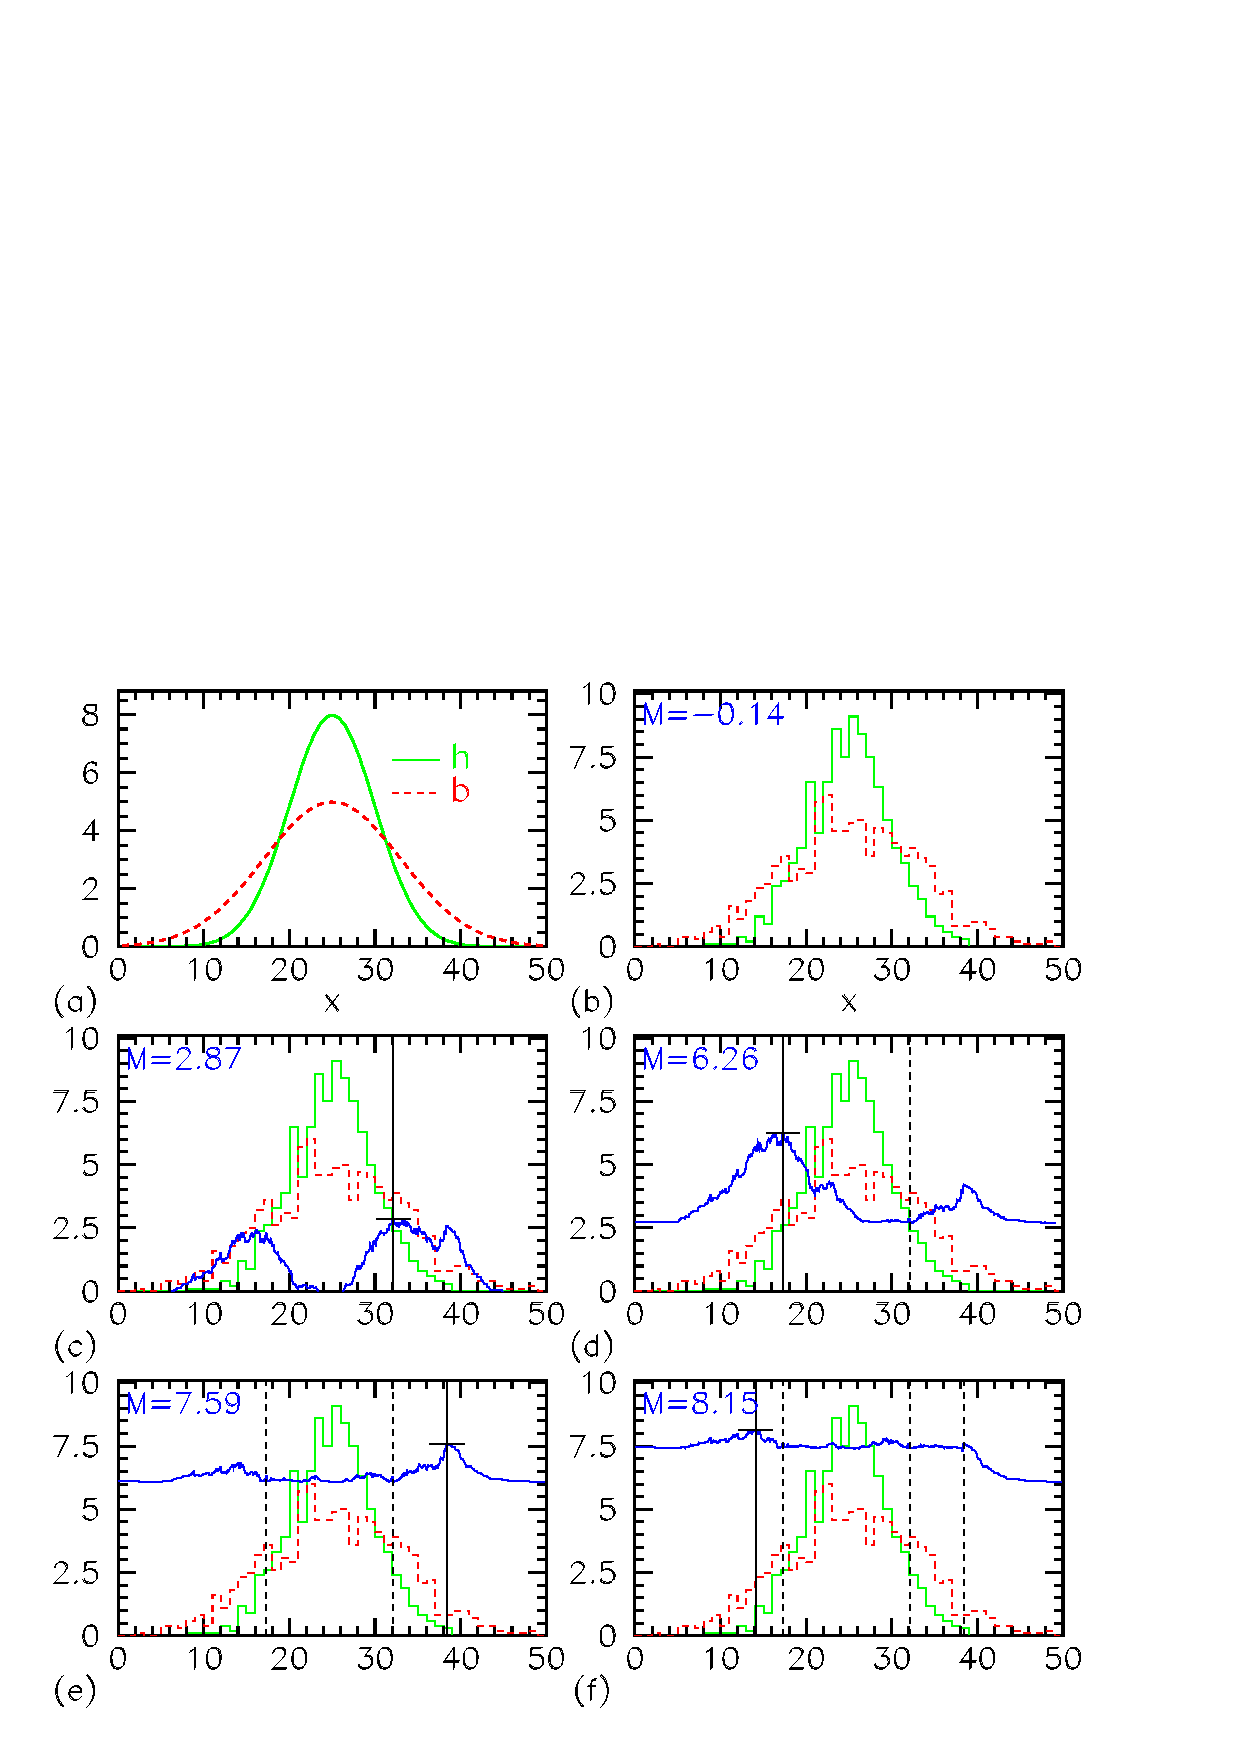
\includegraphics{figures/plot02.pdf} \else 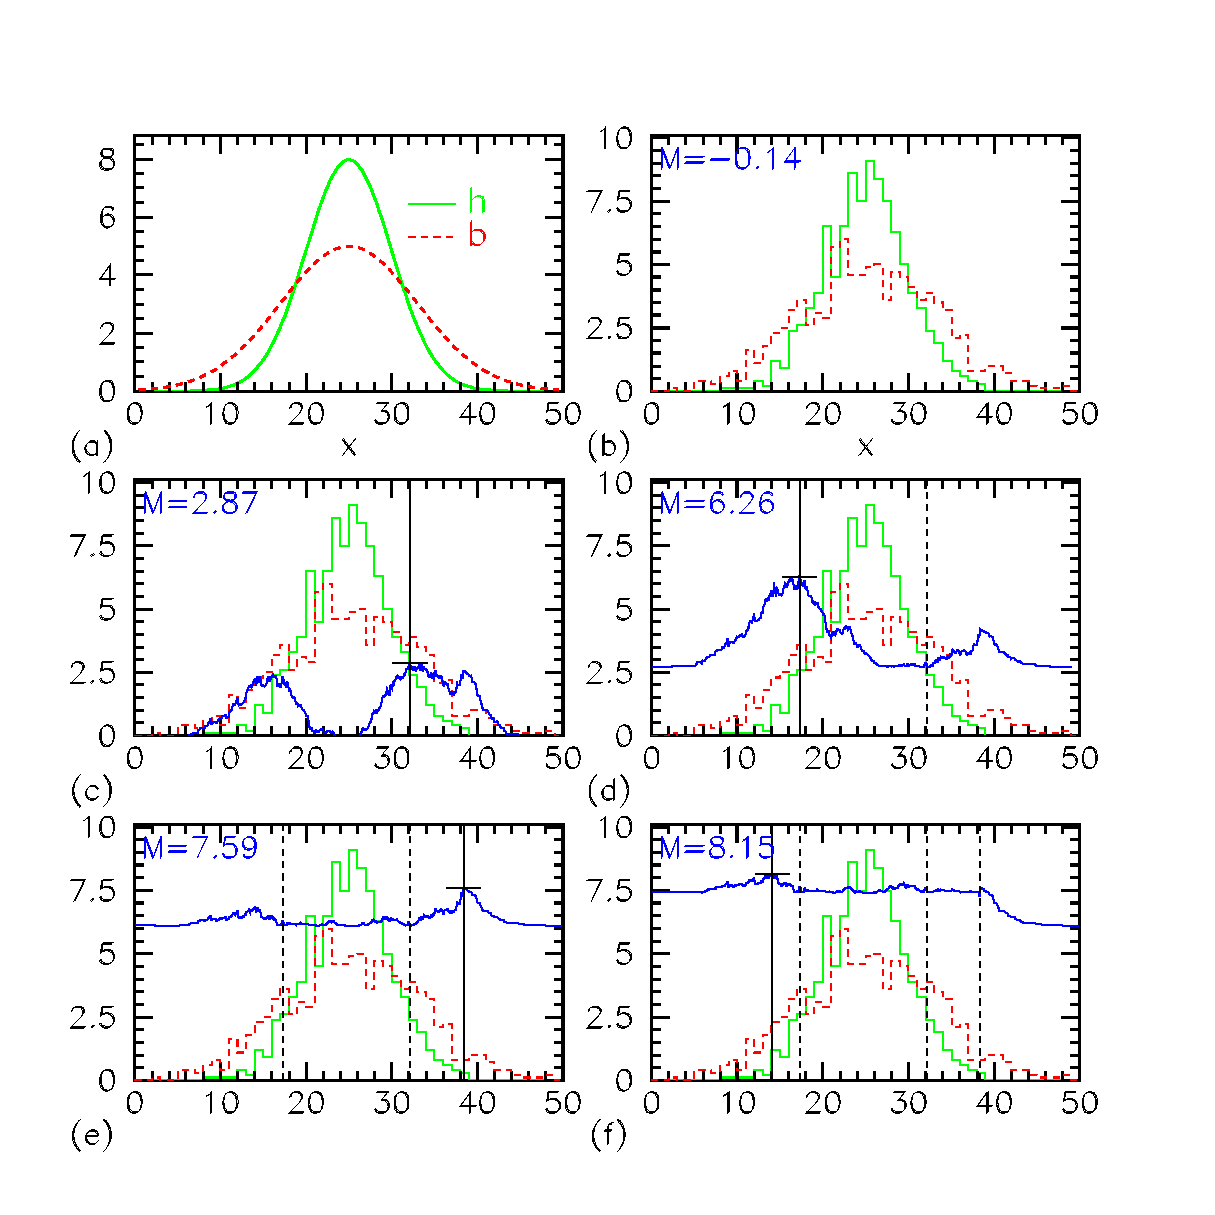
\includegraphics{figures/plot02.eps} \fi }
\vskip -0.2in 
\caption{A second example of using ${\cal M}$ to choose a reasonable set of bins.  The analytical predictions (a) of $h$ (solid) and $b$ (dashed) are unknown, but can be estimated (b) with Monte Carlo.  The vertical axis in (a) and (b) represents the number of data points expected per unit of $x$; the vertical axis in (c)--(f) has units of evidence, and represents the figure of merit ${\cal M}$ if an additional bin edge is placed at $x$.  The successive placing of bin edges at maximal points of ${\cal M}$ is shown in (c)--(f).}
\label{fig:Example2}
\end{figure}

Treating the range $0<x<\infty$ as a single bin, the initial figure of merit is calculated to be negative (${\cal M} = 0 - {\cal P} = -0.14$).  The sequential addition of bin edges at $x=32.1$, $x=17.3$, $x=38.4$, and $x=14.1$ is shown in Figs.~\ref{fig:Example2}(c)--(f), raising the figure of merit to ${\cal M} = 8.15$.  The algorithm proceeds to add additional edges at $x=29.5$, 23.1, 21.0, 20.2, 27.9, 21.2, 29.7, and 20.5 before halting, achieving a final figure of merit ${\cal M}=8.9$.  The resulting bins are concentrated in the regions $x\approx 20$ and $x\approx 30$, where $h(x)$ and $b(x)$ cross.  

The resulting figure of merit ${\cal M}=8.9$ indicates that the actual experiment will on average produce results that favor one hypothesis over the other by nearly nine orders of magnitude.  Running $10^4$ pseudo experiments confirms this result.  If $h$ is correct, evidence in favor of $h$ of 6.4 is achieved on average; if $b$ is correct, evidence in favor of $b$ of 10.7 is achieved on average.  The difference between the mean of 8.5 and ${\cal M}=8.9$ arises from the fact that the ensemble of pseudo experiments is distributed according to the true $h$ and $b$, while the figure of merit must be calculated from the given points $\{ h_i \}$ and $\{ b_j \}$. 

\section{\label{sec:MultivariateCase}Multivariate case}

In the multivariate case, the hypotheses $h$ and $b$ predict a set of observables $\vec{x}$.  The extension of the above prescription to the case of multiple observables is immediate.  A grid of bins in the $d$-dimensional space is defined by $(d-1)$-dimensional partitions of the form (observable) = (constant).  (The grid in the 1-dimensional Example \#1 above was defined by 0-dimensional partitions (points) at $x=18.1$, $x=23.1$, and so forth.)  The partitions are again chosen to maximize ${\cal M}$, with each successive edge possibly determined by any one of the observables.  The resulting grid of bins is neither regular nor equally divided in each observable, but rather adapted to maximally distinguish between $h$ and $b$, within the limits imposed by the constraint that the partitions be of the form (observable) = (constant).

This constraint is sufficiently tight that an alternative approach is advocated.  The multivariate problem is first reduced to the univariate case using any of a number of classification algorithms, and the procedure described above is then applied to the resulting one-dimensional problem.  For definiteness, one such classification algorithm is described here.  Others may be used.

\subsection{Reduction to limited dimensionality}

The first step is the reduction of a potentially large variable space to a space of limited dimensionality $d$.  The dimensionality of this space is dictated by the number $n_\text{MC}$ of Monte Carlo points $\{ h_i \}$ and $\{ b_j \}$ at hand.  A reasonable rule of thumb is to choose $d = \floor{\log_{10}{n_\text{MC}}}$, where $\floor{\cdot}$ is the floor operator, denoting the largest integer not exceeding its argument.  The motivation for this rule lies in the observation that it is difficult to construct a meaningful one-dimensional histogram with fewer than $\approx 10$ points, and in general difficult to construct a meaningful $d$-dimensional histogram with fewer than $\approx 10^d$ points.~\footnoteParenthetical{The choice of 10 can be argued up to, but not much beyond, a factor of two.}

From the observables $\vec{x}$ we generate a possibly long but finite list of relevant variables $\vec{x}'$.  The variables $\vec{x}'$ should be combinations of the observables $\vec{x}$ that lend themselves to the scientist's intuition.

The variables $\vec{x}'$ are then ordered according to decreasing maximal discrepancy between the cumulative distributions predicted by $h$ and by $b$.  This ordering puts variables in which the shapes of the predictions from $h$ and $b$ are very different at the top of the list, and variables in which the shapes of the predictions from $h$ and $b$ are very similar at the bottom.  Beginning then with the first variable in this ordering and continuing until $d$ variables have been chosen, the variable is added to those we consider unless the smallest eigenvalue of the correlation matrix of this variable and the $q-1$ variables already chosen is smaller than $1/q$. \footnoteIgnore{The use of a robust correlation matrix, in which outliers are removed and the L$^1$ norm is used instead of the L$^2$ norm, is preferred in practice.} The idea behind this prescription is that the $d$ variables in which $h$ and $b$ differ most should be used, avoiding variables that provide redundant information.  Variables not chosen by this procedure are discarded from $\vec{x}'$.

\subsection{Reduction to a single dimension}

The method of Probability Density Estimation~\cite{PDE} is used to reduce the problem to a single dimension.  Given the points $\{ h_i \}$ and $\{ b_j \}$ in the variables $\vec{x}'$, we construct the densities
\begin{equation}
\label{eqn:PDEh}
p(\vec{x}'|h) =   \frac{\sum_i{ w_i \exp{\left( - (\vec{x}'-\vec{x}'_i)^T {\sigma_h}^{-1} (\vec{x}'-\vec{x}'_i) / 2 {h^\star_h}^2 \right)}}}{\sqrt{2 \pi \abs{\sigma_h}} h^\star_h \, { \sum_i{w_i} }}
\end{equation}
and
\begin{equation}
\label{eqn:PDEb} 
p(\vec{x}'|b) =  \frac{\sum_j{ w_j \exp{\left( - (\vec{x}'-\vec{x}'_j)^T {\sigma_b}^{-1} (\vec{x}'-\vec{x}'_j) / 2 {h^\star}^2 \right)}}}{\sqrt{2 \pi \abs{\sigma_b}} h^\star_b \, { \sum_j{w_j} }},
\end{equation}
where $\sigma_h$ and $\sigma_b$ are the $d \times d$ covariance matrices of the points $\{ h_i \}$ and $\{ b_j \}$, with determinants $\abs{\sigma_h}$ and $\abs{\sigma_b}$; $\vec{x}'_i$ and $\vec{x}'_j$ are the positions of the points $\{ h_i \}$ and $\{ b_j \}$ in the variables $\vec{x}'$; $(\cdot)^T$ denotes transpose; $w_i$ and $w_j$ are the weights of the points $\{ h_i \}$ and $\{ b_j \}$; and 
\begin{gather}
h^\star_h = (\sum_i{w_i} / \sum_i{w_i^2})^{-1/(d+4)} \\ 
h^\star_b = (\sum_j{w_j} / \sum_j{w_j^2})^{-1/(d+4)}
\end{gather} 
\cite{Scott,Wand} are two parameters determining the smoothness of the resulting distributions.  The values of these parameters are intentionally chosen to modestly over-smooth both distributions.~\footnoteParenthetical{Improved algorithms for kernel density estimation, some of which adjust the smoothing parameters adaptively, exist in the literature.  The simplest estimator is presented here.}

The densities $p(\vec{x}'|h)$ and $p(\vec{x}'|b)$ are used to define a discriminant
\begin{equation}
\label{eqn:Discriminant}
D(\vec{x}') = \frac{ p(\vec{x}'|h) }{ p(\vec{x}'|h) + p(\vec{x}'|b) }.
\end{equation}
The range of $D(\vec{x}')$ is the interval $(0,1)$; $D$ is large in regions populated by $h$ but not by $b$; $D$ is small in regions populated by $b$ but not by $h$.  We compute for each of the points $\{ h_i \}$ and $\{ b_j \}$ the variables $D(\vec{x}'_i)$ and $D(\vec{x}'_j)$. \footnoteParenthetical{The $i^{th}$ event is removed from the sum in Eq.~(\ref{eqn:PDEh}) when computing $D(\vec{x}'_i)$; similarly, the $j^{th}$ event is removed from the sum in Eq.~(\ref{eqn:PDEb}) when computing $D(\vec{x}'_j)$.}

The densities $p(\vec{x}'|h)$ and $p(\vec{x}'|b)$ can in principle be used to compute an unbinned likelihood ratio.  In practice, this ratio can suffer from systematic dependence on the details of the smoothing procedure.  In Example \#2 above, the use of over-smoothed densities causes a bias in favor of hypotheses predicting narrow Gaussians, while the use of under-smoothed densities causes undesired dependence on the small-scale structure of the points $\{ h_i \}$ and $\{ b_j \}$.  The calculation of a binned likelihood ratio in the resulting discriminant reduces the dependence on the smoothing procedure, and has the additional advantage that it can be applied to the output of other classification algorithms.

%\vskip 30pt The point of this section, which has been largely review, is to recall a definite prescription for reducing the problem of optimally binning a multivariate likelihood to the problem of optimally binning a univariate likelihood.

\begin{figure}[tbh]
\resizebox{\figuresize}{!}{\hskip -0.5cm \ifpdf 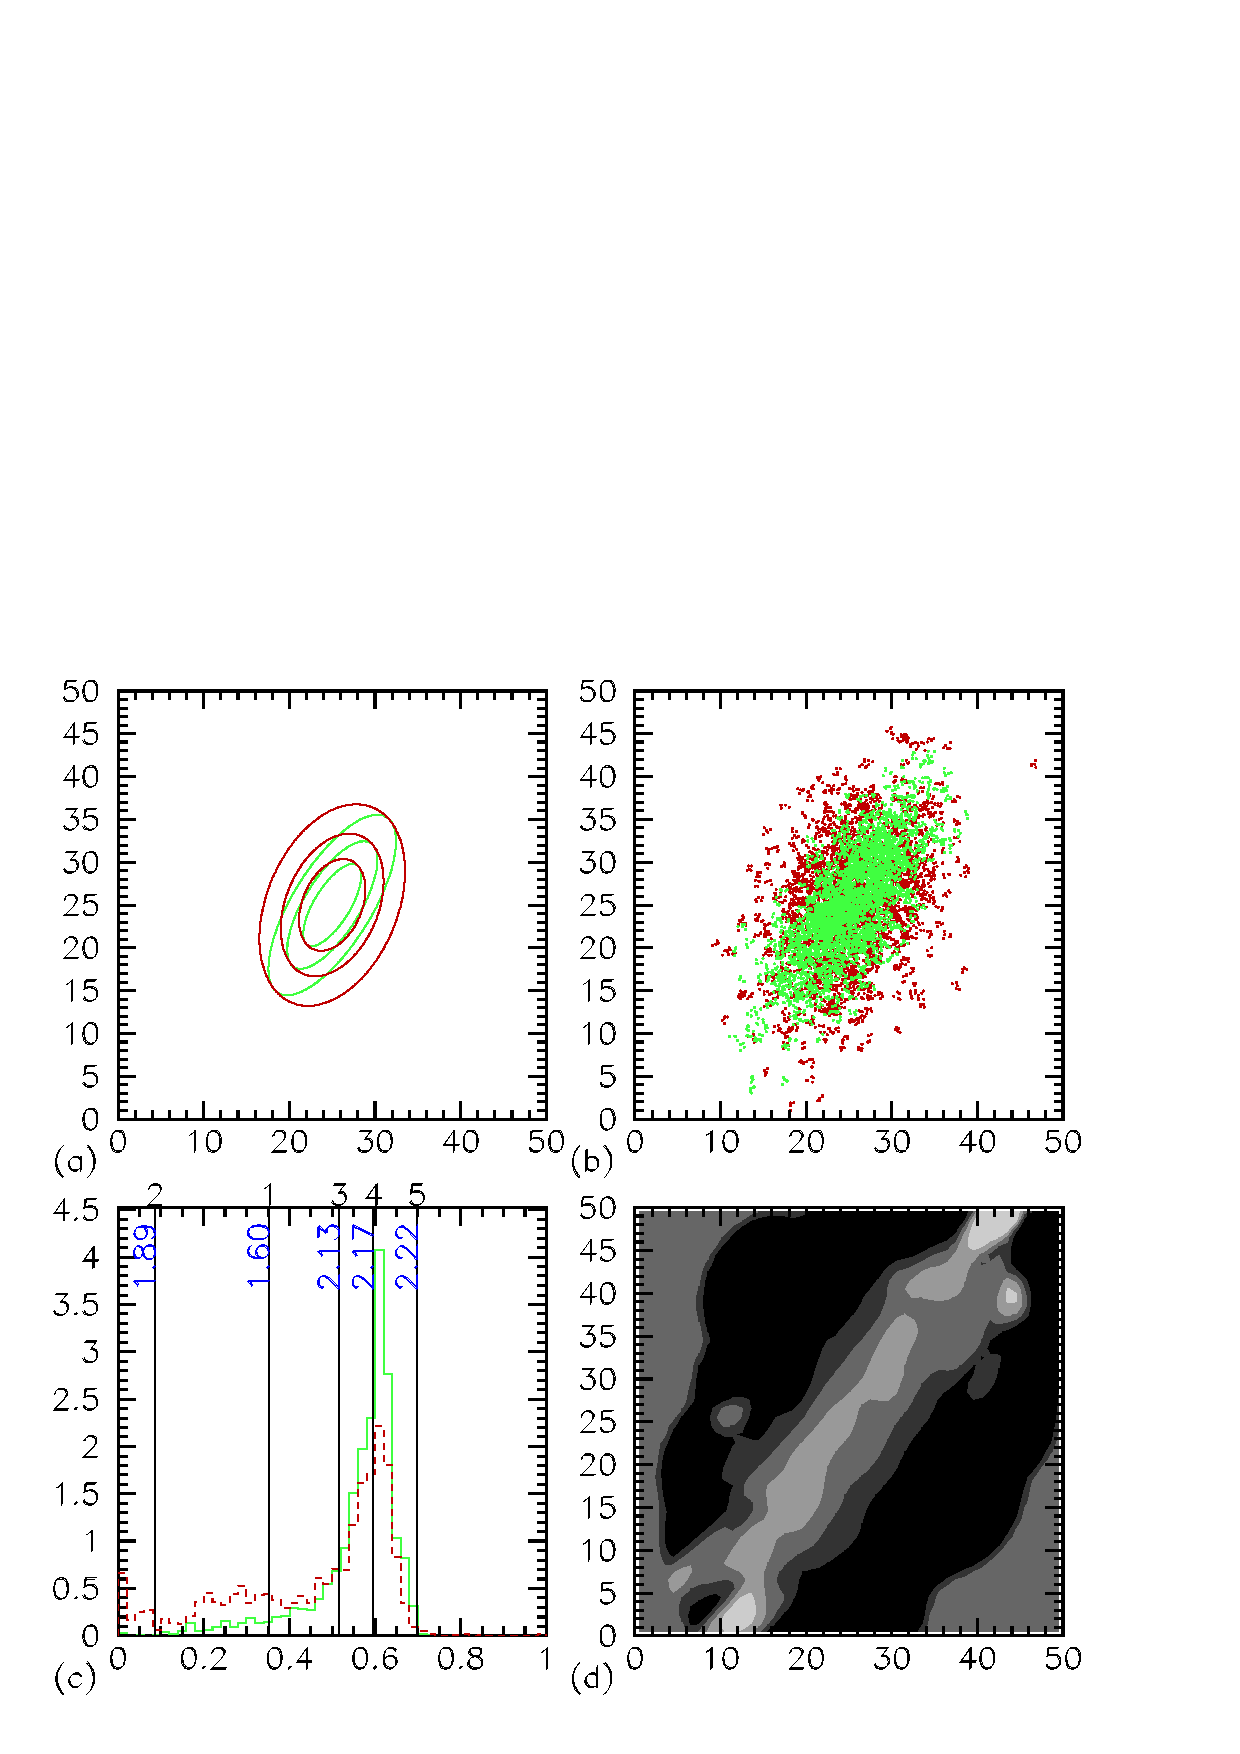
\includegraphics{figures/plot03.pdf} \else 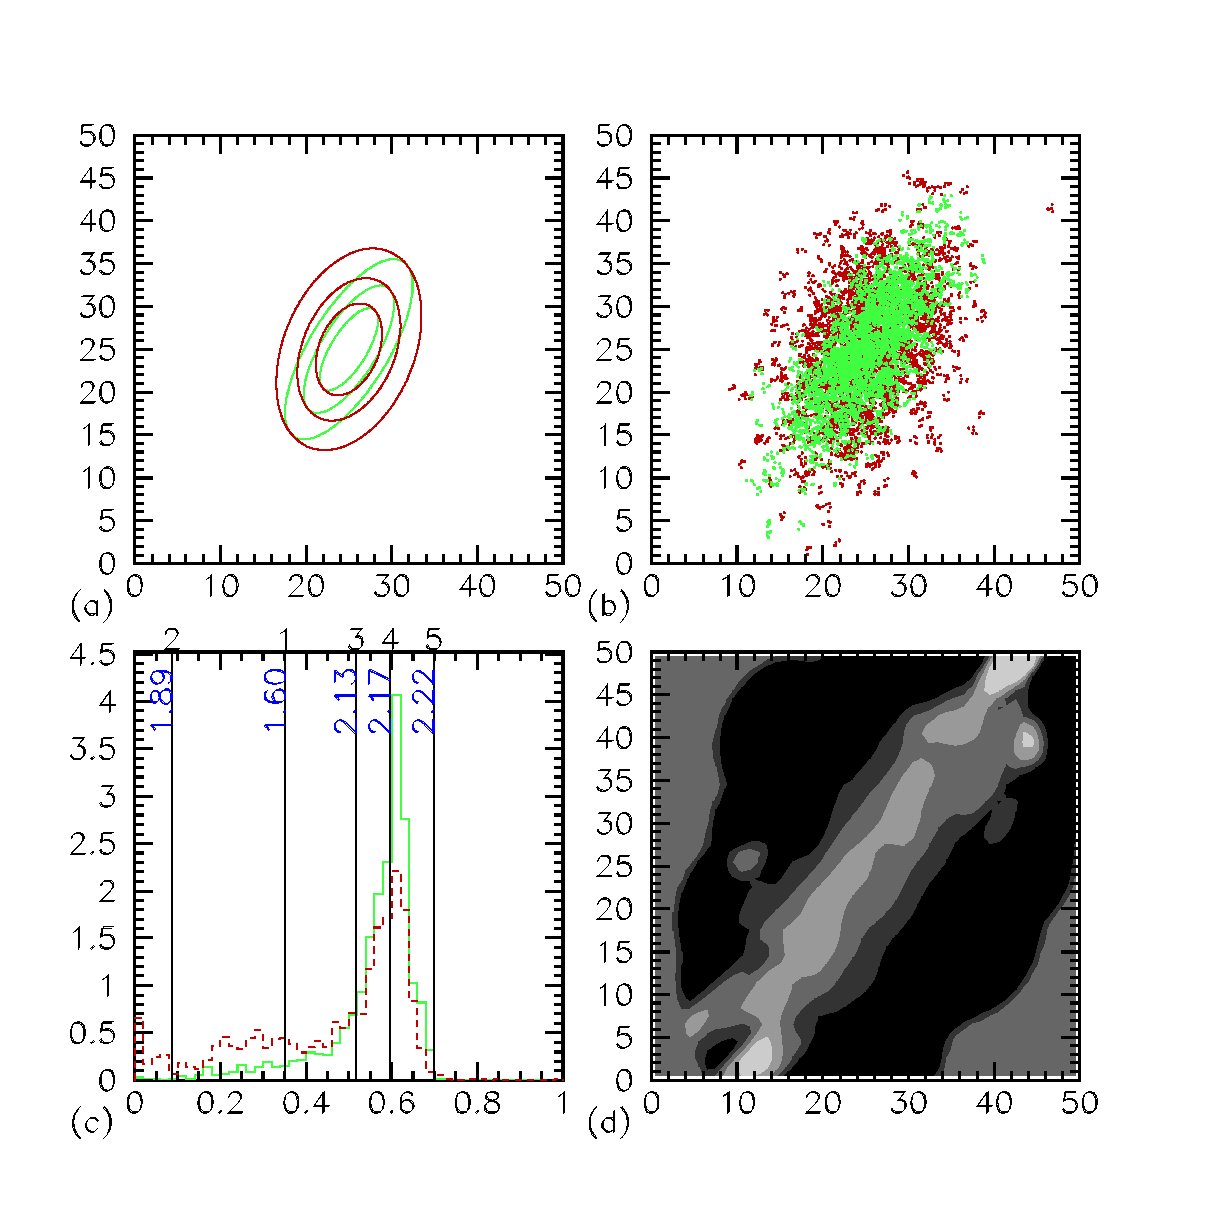
\includegraphics{figures/plot03.eps} \fi }
\vskip -0.2in 
\caption{A multivariate example.  Contours of the true predictions of $h$ (light three ellipses, larger correlation) and $b$ (dark three ellipses, smaller correlation) are shown in (a).  Points pulled from $h$ (light dots) and $b$ (dark dots) are displayed in (b).  A discriminant is constructed from probability densities estimated from the points in (b), which map the points from $h$ (solid) and $b$ (dashed) onto the unit interval in (c).  The positions of successive bin edge placements are shown by numbered lines.  Along each line is given the figure of merit achieved after that partition is added.  The partitions in the unit interval in turn partition the original space, shown in the contours of (d).  The lightest region corresponds to the bin $(0.70,1.00)$; the darkest to the bin $(0.00,0.09)$.}
\label{fig:Example3}
\end{figure}

\subsection{Example \#3: Multivariate Gaussians with different covariance}

Example \#2 of Sec.~\ref{sec:Examples} can be extended to the multivariate case in which $h$ and $b$ predict bivariate Gaussian distributions of different covariance.  Figure~\ref{fig:Example3}(a) shows simple contours of the true distributions in the 2-dimensional space $\vec{x}'$, allowing an easy comparison of the covariances.   One thousand points have been randomly drawn from $b(x)$ and from $h(x)$, each with weight 0.01.  The points are displayed in the scatter plot of Fig.~\ref{fig:Example3}(b).

Figure~\ref{fig:Example3}(c) shows the location of the points in the unit interval after forming the discriminant of Eq.~(\ref{eqn:Discriminant}).  The points predicted by $h$ (solid) generally lie to somewhat larger values of the discriminant than do the points predicted by $b$ (dashed), although the difference is not striking.  Successive bin edges are placed in turn at $x=0.36$, $x=0.09$, $x=0.52$, $x=0.59$, and $x=0.70$, achieving a figure of merit of ${\cal M}=2.22$.  The placement of fifteen additional bins raises the figure of merit to 2.5 before the algorithm halts.  

The partitions in the unit interval of Fig.~\ref{fig:Example3}(c) in turn define non-rectangular bins in the original space, shown in Fig.~\ref{fig:Example3}(d).  Each shade corresponds to one of the bins in Fig.~\ref{fig:Example3}(c); darker regions correspond to smaller values of the discriminant, and lighter regions to larger values.  The general flow of the contour edges can be easily understood from the shapes of $h$ and $b$ shown in Figs.~\ref{fig:Example3}(a) and (b).

\section{Summary}

The main result of this article is the proposal that the figure of merit ${\cal M}$ defined by Eq.~(\ref{eqn:FigureOfMerit}) be used to determine the placement of bins in the calculation of likelihood ratios.  The results of this proposal have been examined in several limiting cases.  Simple analytic expressions for the figure of merit and related quantities have been derived in appropriate high statistics limits.  The familiar maximization of $s/\sqrt{b}$ is derived as a special case.  The reasonable consequences of the proposal have been illustrated in two univariate examples.  Extension to the multivariate case has been treated by employing a rule for the selection of variables and kernel density estimation to reduce the problem to the univariate case.  Intuitive results are obtained in a multivariate generalization of the second univariate example.

The calculation of likelihood ratios is common practice in the physical and social sciences; we expect the procedure outlined here to have widespread application.


\bibliography{optimalBinning}

%===============================================================
\end{document}

